% 2018 全国Ⅰ卷 文18：平行四边形 ABCM 沿 AC 折起，M 到达 D（AB⊥DA）
% Q 在 AD 上，P 在 BC 上；虚线 M 为折叠前位置
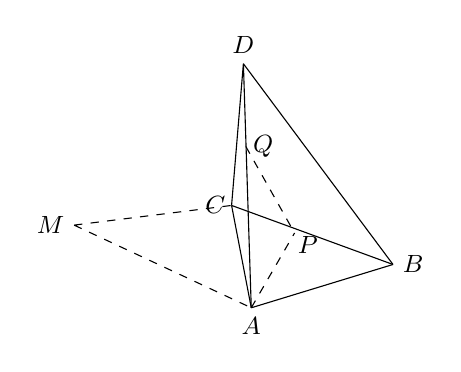
\begin{tikzpicture}[scale=1.0, font=\small]
  \coordinate (A) at (2.6,0);
  \coordinate (B) at (4.4,0.55);
  \coordinate (C) at (2.35,1.3);
  \coordinate (M) at (0.35,1.05);
  \coordinate (D) at (2.5,3.1);
  \coordinate (Q) at (2.53,2.05);
  \coordinate (P) at (3.15,0.95);
  \draw (A) -- (B);
  \draw (A) -- (C)  (B) -- (C);
  \draw (C) -- (D)  (A) -- (D);
  \draw (D) -- (B);
  \draw[dashed] (M) -- (A)  (M) -- (C);
  \draw[dashed] (A) -- (P)  (Q) -- (P);
  \node[below] at (A) {$A$};
  \node[right] at (B) {$B$};
  \node[left, inner sep=2pt] at (C) {$C$};
  \node[left] at (M) {$M$};
  \node[above] at (D) {$D$};
  \node[right, inner sep=2.5pt] at (Q) {$Q$};
  \node[below right, inner sep=1pt] at (P) {$P$};
\end{tikzpicture}
